\subsection{Stubbornness and social power in the FDG model}
\label{subsec:fdg-stub}

In the FDG model the simplest way to account for stubbornness is the self-weight
$a_{ii}$, i.e.\ the weight of the self-loop of agent $i$. This section studies how
self-weights, and stubborn agents in particular, affect the two aspects introduced in
Section~\ref{subsec:fdg-intro}: whether the group reaches an agreement, and how the
social power is distributed among the agents.

All the examples use the two networks of Figure~\ref{fig:networks}, both with $n = 6$
agents: in the \emph{directed cycle} each agent is influenced only by the next one,
$a_{i,i+1} = 1$; in the \emph{bidirectional ring} by its two neighbours,
$a_{i,i-1} = a_{i,i+1} = 1/2$ (indices modulo $6$). Socially, in the first network
everyone listens to a single person, in the second to the two people next to them.
Without self-loops both digraphs are strongly connected and periodic, with period $6$
for the directed cycle and $2$ for the bidirectional ring, whose cycles all have even
length: neither network reaches an agreement (case~(ii) of Table~\ref{tab:rosetta}).
Both matrices are doubly-stochastic, so $w = \frac{1}{6}\mathbf{1}_6$ is the left
eigenvector associated with the eigenvalue $1$: no agent is favoured by the structure
of the network, and any asymmetry in the social power will be due only to the
self-weight added to agent~$1$.
% REVISED (2026-10-28, review): shortened, same content. Was:
% All the examples use the two networks of Figure~\ref{fig:networks}, both with $n = 6$
% agents. In the \emph{directed cycle} each agent is influenced only by the next one,
% $a_{i,i+1} = 1$; in the \emph{bidirectional ring} each agent is influenced by its two
% neighbours with equal weights, $a_{i,i-1} = a_{i,i+1} = 1/2$ (indices modulo $6$).
% Socially, in the first network everyone listens to a single person, while in the second
% everyone listens to the two people next to them. Without self-loops both digraphs are
% strongly connected and periodic: the directed cycle has a single cycle, of length $6$,
% while every cycle of the bidirectional ring has even length, so its period is $2$.
% Hence neither network reaches an agreement (case~(ii) of Table~\ref{tab:rosetta}).
% Moreover, both matrices are doubly-stochastic, so $w = \frac{1}{6}\mathbf{1}_6$ is the
% left eigenvector associated with the eigenvalue $1$: no agent is favoured by the
% structure of the network, and any asymmetry in the social power will be due only to
% the self-weight added to agent~$1$.

\begin{figure}[H]
  \centering
  \begin{tikzpicture}[baseline=(c.base)]
    \foreach \i in {1,...,6} {
      \node[agent] (d\i) at ({90-60*(\i-1)}:1.3) {\i};
    }
    \node (c) at (0,0) {};
    \foreach \i/\j in {2/3,3/4,4/5,5/6,6/1} {
      \draw[edge] (d\i) -- (d\j);
    }
    \draw[edge] (d1) -- node[weight, above right] {$1-t$} (d2);
    \draw[selfloop, dashed] (d1) to node[weight, above] {$t$} (d1);
    % REVISED (2026-10-28): the edge 1 -> 2 is now drawn separately with its weight 1-t
    % (was part of the \foreach list 1/2,2/3,...,6/1).
    \node at (0,-2.0) {\small (a) directed cycle};
  \end{tikzpicture}
  \hspace{1.5cm}
  \begin{tikzpicture}[baseline=(c.base)]
    \foreach \i in {1,...,6} {
      \node[agent] (b\i) at ({90-60*(\i-1)}:1.3) {\i};
    }
    \node (c) at (0,0) {};
    \foreach \i/\j in {2/3,3/4,4/5,5/6} {
      \draw[edge] (b\i) to[bend left=12] (b\j);
      \draw[edge] (b\j) to[bend left=12] (b\i);
    }
    \draw[edge] (b2) to[bend left=12] (b1);
    \draw[edge] (b6) to[bend right=12] (b1);
    \draw[edge] (b1) to[bend left=12] node[weight, above right] {$\frac{1-t}{2}$} (b2);
    \draw[edge] (b1) to[bend right=12] node[weight, above left] {$\frac{1-t}{2}$} (b6);
    \draw[selfloop, dashed] (b1) to node[weight, above] {$t$} (b1);
    % REVISED (2026-10-28): the edges 1 -> 2 and 1 -> 6 are now drawn separately with
    % their weight (1-t)/2 (were part of the \foreach list 1/2,...,6/1).
    \node at (0,-2.0) {\small (b) bidirectional ring};
  \end{tikzpicture}
  \caption{The two networks used in Sections~\ref{subsec:fdg-stub}
  and~\ref{sec:fj}. An edge $i \to j$ means that agent $i$ is influenced by agent $j$.
  In (a) all edges have weight $1$, in (b) all edges have weight $1/2$. The dashed
  self-loop of agent~$1$, of weight $t$, is the only modification considered: the
  other edges of agent~$1$ are scaled by $1-t$, as marked
  (equation~\eqref{eq:self-weight}).}
  % REVISED (2026-10-28): added "as marked" (the weights of the edges of agent 1 are now
  % written on the figure).
  \label{fig:networks}
\end{figure}

\subsubsection{Modelling stubbornness: self-weights and stubborn agents}
\label{subsubsec:fdg-stub-model}

The self-weight $a_{ii}$ is the weight that agent $i$ gives to its own \emph{current}
opinion~\cite{bullo2024lns}; it indicates how open the agent is to the opinions of the
others~\cite{proskurnikov2017tutorial}. An agent with $a_{ii} = 0$ is open-minded and
relies completely on the others; an agent with a positive self-weight changes its
opinion more slowly, but it still moves towards the opinions it listens to. In social
terms, a self-weight is a form of inertia, not an anchor to a fixed opinion.

\begin{definition}[Stubbornness~\cite{proskurnikov2017tutorial}]
\label{def:stubborn}
% REVISED (2026-10-24): definition now exactly as Definition 16 of the tutorial; the
% FDG characterization (a_ii = 1) is moved to the text below.
An agent is said to be \emph{stubborn} if its opinion remains unchanged independent
of the others' opinions.
\end{definition}

If the opinions obey the FDG model, then agent $i$ is stubborn, $x_i(k) \equiv x_i(0)$,
if and only if $a_{ii} = 1$~\cite{proskurnikov2017tutorial} (and hence $a_{ij} = 0$
for all $j \neq i$, since $A$ is row-stochastic).

Stubbornness is therefore the extreme case of the self-weight, and there is no
intermediate degree of it: an agent with $0 < a_{ii} < 1$ is not stubborn, it only has
a positive self-weight.

In the digraph, a stubborn agent has no edges towards the other agents: it is
influenced by nobody, while the agents that listen to it keep doing so. Hence it forms
a strongly connected component made of a single node, which is a sink of $C(G)$ and is
aperiodic because of its self-loop. If, in addition, every agent is influenced by the
stubborn agent $i$, directly or through intermediaries, then $i$ is the only globally
reachable node, and Theorem~\ref{thm:consensus} gives $w = e_i$: the whole group
converges to the initial opinion of the stubborn agent (see
also~\cite{proskurnikov2017tutorial}).

To move continuously from no self-weight to stubbornness, we modify only the row of
agent~$1$. Given a row-stochastic matrix $A$ with $a_{11} = 0$, as in both networks of
Figure~\ref{fig:networks}, we replace its first row by
\begin{equation}\label{eq:self-weight}
  a_1(t)^\top = (1-t)\, a_1^\top + t\, e_1^\top, \qquad t \in [0,1],
\end{equation}
where $e_1$ is the first vector of the canonical basis, leaving the other rows
unchanged: agent~$1$ gives weight $t$ to itself and splits the remaining weight $1-t$
among the agents it listened to before, in the same proportions, as marked in
Figure~\ref{fig:networks}. Thus $t = a_{11}$: $t = 0$ is the original network and
$t = 1$ makes agent~$1$ stubborn. In the following we consider $t = 0$, $1/2$ and $1$.
% REVISED (2026-10-28, review): shortened; the explicit first rows are now written on Figure 1. Was:
% where $e_1$ is the first vector of the canonical basis, and leave the other rows
% unchanged. Agent~$1$ gives weight $t$ to itself and splits the
% remaining weight $1-t$ among the agents it listened to before, in the same
% proportions. The parameter $t$ is thus the self-weight $a_{11}$: $t = 0$ is the
% original network, $0 < t < 1$ gives agent~$1$ a positive self-weight, and $t = 1$
% makes agent~$1$ stubborn. For the directed cycle the first row becomes
% $(t,\, 1-t,\, 0,\, 0,\, 0,\, 0)$; for the bidirectional ring it becomes
% $(t,\, \frac{1-t}{2},\, 0,\, 0,\, 0,\, \frac{1-t}{2})$. In the following we consider
% the three values $t = 0$, $t = 1/2$ and $t = 1$.

\subsubsection{Self-weights, stubbornness and convergence}
\label{subsubsec:fdg-stub-conv}

The three values of $t$ correspond to three different cases of the Rosetta stone.
\begin{itemize}
  \item $t = 0$: both digraphs are strongly connected and periodic, so neither
        network converges (case~(ii)).
  \item $0 < t < 1$: agent~$1$ still listens to its neighbours with total weight
        $1-t > 0$, so the digraph stays strongly connected, and the self-loop of
        agent~$1$ is a cycle of length $1$, so the digraph becomes aperiodic. By
        Corollary~\ref{cor:primitive-selfloop} the matrix is primitive, and the group reaches a
        consensus (case~(i)).
  \item $t = 1$: agent~$1$ is stubborn and influences every other agent through the
        cycle, so it is the only globally reachable node
        (Section~\ref{subsubsec:fdg-stub-model}) and the group reaches a consensus on
        $x_1(0)$ (case~(iii)).
% REVISED (2026-10-28, review): shortened, same content. Was:
%   \item $t = 1$: agent~$1$ is stubborn. In both networks every other agent is
%         influenced by agent~$1$ through the cycle, directly or through intermediaries,
%         so by the discussion in Section~\ref{subsubsec:fdg-stub-model} agent~$1$ is the
%         only sink of $C(G)$ and the only globally reachable node, so the group reaches a consensus on its initial
%         opinion $x_1(0)$ (case~(iii)).
\end{itemize}

The same picture can be read on the spectrum of $A(t)$. For $t = 0$ the spectrum is the
set of the sixth roots of unity for the directed cycle and
$\{1, \frac{1}{2}, \frac{1}{2}, -\frac{1}{2}, -\frac{1}{2}, -1\}$ for the bidirectional
ring: in both cases some eigenvalues different from $1$ lie on the unit circle, and
they cause the oscillations. For $t > 0$ all the eigenvalues different from $1$ lie
strictly inside the unit disk, and the group converges; for $t = 1/2$ the largest of
their moduli is $\approx 0.92$ on the directed cycle and $\approx 0.90$ on the
bidirectional ring. For $t = 1$ the directed cycle is left with the eigenvalue $0$, of
multiplicity $5$, which is why its consensus is reached in a finite number of steps.
% REVISED (2026-10-28, review): the characteristic polynomials and the lists of eigenvalues are summarized (FDG part to be kept essential); the moduli 0.92 and 0.90 are those of the removed lists for t = 1/2. Was:
% The same picture can be read on the spectrum of the matrix. For the directed cycle the
% characteristic polynomial is
% \[
%   p(\lambda) = (\lambda - 1)\,\big[\lambda^5 + (1-t)(\lambda^4 + \lambda^3 + \lambda^2
%   + \lambda + 1)\big].
% \]
% Apart from $\lambda_1 = 1$, the eigenvalues are the roots of a polynomial of degree $5$,
% which for a generic $t$ have no closed-form expression; for the three values of $t$
% they are
% \begin{itemize}
%   \item $t = 0$: $\lambda_1 = 1$, $\lambda_{2,3} = \frac{1}{2} \pm \frac{\sqrt{3}}{2}\,i$,
%         $\lambda_{4,5} = -\frac{1}{2} \pm \frac{\sqrt{3}}{2}\,i$, $\lambda_6 = -1$
%         (the sixth roots of unity, all on the unit circle);
%   \item $t = 1/2$: $\lambda_1 = 1$, $\lambda_{2,3} \approx 0.535 \pm 0.751\,i$,
%         $\lambda_{4,5} \approx -0.373 \pm 0.759\,i$, $\lambda_6 \approx -0.823$;
%   \item $t = 1$: $\lambda_1 = 1$, $\lambda_2 = \dots = \lambda_6 = 0$.
% \end{itemize}
% For the bidirectional ring the characteristic polynomial is
% \[
%   p(\lambda) = (\lambda - 1)\big(\lambda - \tfrac{1}{2}\big)
%   \big(\lambda + \tfrac{1}{2}\big)\Big[\lambda^3 + (1-t)\lambda^2
%   - \tfrac{2t+1}{4}\,\lambda + \tfrac{t-1}{4}\Big].
% \]
% The eigenvalues $1$ and $\pm\frac{1}{2}$ do not depend on $t$, while the other three are
% the roots of the cubic factor, whose closed-form expression in $t$ is too involved to be
% informative; for the three values of $t$ the eigenvalues are
% \begin{itemize}
%   \item $t = 0$: $\lambda_1 = 1$, $\lambda_{2,3} = \frac{1}{2}$,
%         $\lambda_{4,5} = -\frac{1}{2}$, $\lambda_6 = -1$ (on the unit circle);
%   \item $t = 1/2$: $\lambda_1 = 1$, $\lambda_2 \approx 0.623$, $\lambda_3 = \frac{1}{2}$,
%         $\lambda_4 \approx -0.223$, $\lambda_5 = -\frac{1}{2}$, $\lambda_6 \approx -0.901$;
%   \item $t = 1$: $\lambda_1 = 1$, $\lambda_2 = \frac{\sqrt{3}}{2}$,
%         $\lambda_3 = \frac{1}{2}$, $\lambda_4 = 0$, $\lambda_5 = -\frac{1}{2}$,
%         $\lambda_6 = -\frac{\sqrt{3}}{2}$.
% \end{itemize}
% In both networks, for $t = 0$ some eigenvalues different from $1$ lie on the unit
% circle, and they cause the oscillations; for $t > 0$ all the eigenvalues different
% from $1$ lie strictly inside the unit disk, and the group converges. For $t = 1$ the
% directed cycle is left with the eigenvalue $0$ only, which is why its convergence is
% reached in a finite number of steps.

Figure~\ref{fig:fdg-conv} shows the opinions $x_i(k)$ in the six cases. For $t = 0$
the opinions keep rotating along the directed cycle and oscillating between two
configurations on the bidirectional ring. For $t = 1/2$ both networks reach a consensus
on a weighted average of all the initial opinions (Section~\ref{subsubsec:fdg-stub-power}).
For $t = 1$ both reach $x_1(0)$, in different ways: in the directed cycle the opinion of
agent~$1$ is copied backwards along the chain, one agent per step, and the consensus is
reached after $n - 1 = 5$ steps; in the bidirectional ring the opinions approach
$x_1(0)$ gradually, the neighbours of agent~$1$ first.
% REVISED (2026-10-28, review): shortened, same content. Was:
% Figure~\ref{fig:fdg-conv} shows the opinions $x_i(k)$ in the six cases. For $t = 0$
% the opinions keep rotating along the directed cycle and keep oscillating between two
% configurations on the bidirectional ring. For $t = 1/2$ both networks reach a consensus
% whose value is a weighted average of all the initial opinions, with weights given by
% the social power (Section~\ref{subsubsec:fdg-stub-power}). For $t = 1$ both networks
% reach a consensus on $x_1(0)$, but in different ways. In the directed cycle every agent
% other than agent~$1$ simply copies the opinion of the next agent, so the opinion of
% agent~$1$ travels backwards along the chain, one agent per step, and the consensus is
% reached exactly after $n - 1 = 5$ steps. In the bidirectional ring every agent averages
% the opinions of its two neighbours, so the opinions approach $x_1(0)$ gradually, the
% neighbours of agent~$1$ first.

\begin{figure}[H]
  \centering
  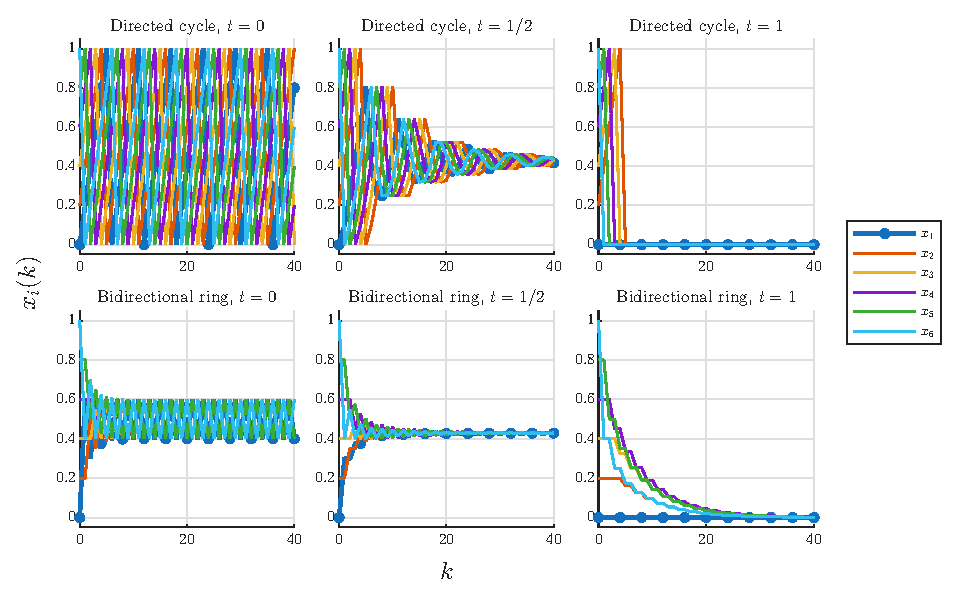
\includegraphics[width=0.94\textwidth]{figures/fdg_convergence.eps}
  \caption{Opinions $x_i(k)$ in the two networks of Figure~\ref{fig:networks}
  (top: directed cycle; bottom: bidirectional ring) for three values of the
  self-weight $t$ of agent~$1$ (columns), with
  $x(0) = (0,\, 0.2,\, 0.4,\, 0.6,\, 0.8,\, 1)^\top$. Agent~$1$ is marked with
  dots.}
  \label{fig:fdg-conv}
\end{figure}

In social terms, a group in which nobody gives weight to its own opinion can keep
passing opinions around forever; a single agent that gives some weight to its current
opinion, without being stubborn, is enough for the whole group to agree, and if that
agent becomes stubborn the agreement is on its own opinion. The network decides only
how this happens: by copying along a chain, or by averaging with the neighbours.
% REVISED (2026-10-28, review): shortened, same content. Was:
% In social terms, a group in which nobody gives weight to its own opinion can keep
% passing opinions around forever. It is enough that a single agent gives some weight to
% its current opinion, without being stubborn, for the whole group to reach an
% agreement. If that agent becomes stubborn, the agreement is reached on its own
% opinion. The structure of the network decides only how this happens: by copying along
% a chain in the directed cycle, by averaging with the neighbours in the bidirectional
% ring.

\subsubsection{Self-weights, stubbornness and social power}
\label{subsubsec:fdg-stub-power}

For $t > 0$ both networks reach a consensus (Section~\ref{subsubsec:fdg-stub-conv}),
so the social power $w$ of Section~\ref{subsubsec:consensus} is well defined, and
Theorem~\ref{thm:consensus} describes how it depends on $t$.
\begin{itemize}
  \item $0 < t < 1$: the digraph is strongly connected, so every agent is globally
        reachable and, by point~(i) of Theorem~\ref{thm:consensus}, every agent has a
        positive social power. Agent~$1$ gives weight to its own opinion, but it does
        not take all the influence: the initial opinion of every agent enters the
        consensus value.
  \item $t = 1$: agent~$1$ is stubborn and is the only globally reachable node, so
        $w = e_1$: the stubborn agent takes all the social power, and the initial
        opinions of the other agents have no effect on the final opinion of the group.
\end{itemize}

Between these two extremes, $w$ is the left eigenvector of $A(t)$ associated with the
eigenvalue $1$, normalized to sum $1$ (condition~(A2) of Theorem~\ref{thm:consensus});
Figure~\ref{fig:fdg-power} reports it for $t \in (0,1]$. Numerically, the social power
of agent~$1$ grows with $t$ towards $1$, while the other agents share the rest equally
($w_1 \approx 0.286$ and $w_i \approx 0.143$ for $i \neq 1$ when $t = 1/2$), with the
same values on the two networks. The bottom panel shows where the group converges, the
consensus value $w^\top x(0)$ (point~(ii) of Theorem~\ref{thm:consensus}): it moves
from the average $0.5$ of the initial opinions, for small $t$, to $x_1(0) = 0$ for
$t = 1$, and it is $\approx 0.429$ for $t = 1/2$, the value reached in
Figure~\ref{fig:fdg-conv}; also this curve is the same on the two networks. In other
words, on these two networks the self-weight of agent~$1$ changes how the opinions
converge, which depends on the network, but not where they converge.
% REVISED (2026-10-28, review): two paragraphs merged and shortened, same content. Was:
% Between these two extremes, the social power can be computed as the left eigenvector
% of $A(t)$ associated with the eigenvalue $1$, normalized so that its entries sum to $1$
% (condition~(A2) of Theorem~\ref{thm:consensus}). Figure~\ref{fig:fdg-power} reports
% the result for $t \in (0,1]$. Numerically, the social power of agent~$1$ grows with $t$
% towards $1$, while the other agents share the remaining social power equally; for
% $t = 1/2$, agent~$1$ has social power $\approx 0.286$ and every other agent
% $\approx 0.143$. Moreover, the computation gives the same values on the two networks.
% In other words, on these two networks the self-weight of agent~$1$ changes how the
% opinions converge, which depends on the network (Figure~\ref{fig:fdg-conv}), but not
% where they converge.
%
% The bottom panel of Figure~\ref{fig:fdg-power} shows where the group converges: by
% point~(ii) of Theorem~\ref{thm:consensus}, the consensus value is $w^\top x(0)$, here
% computed for $x(0) = (0,\, 0.2,\, 0.4,\, 0.6,\, 0.8,\, 1)^\top$, the initial condition of
% Figure~\ref{fig:fdg-conv}. For small $t$ all the agents have almost the same social
% power and the consensus value is close to the average of the initial opinions, $0.5$;
% as $t$ grows, the social power of agent~$1$ grows and the consensus value moves
% towards its initial opinion, $x_1(0) = 0$, which is reached for $t = 1$. For $t = 1/2$
% the consensus value is $\approx 0.429$, the value reached by the trajectories of
% Figure~\ref{fig:fdg-conv}. Also this curve is the same on the two networks.

\begin{figure}[H]
  \centering
  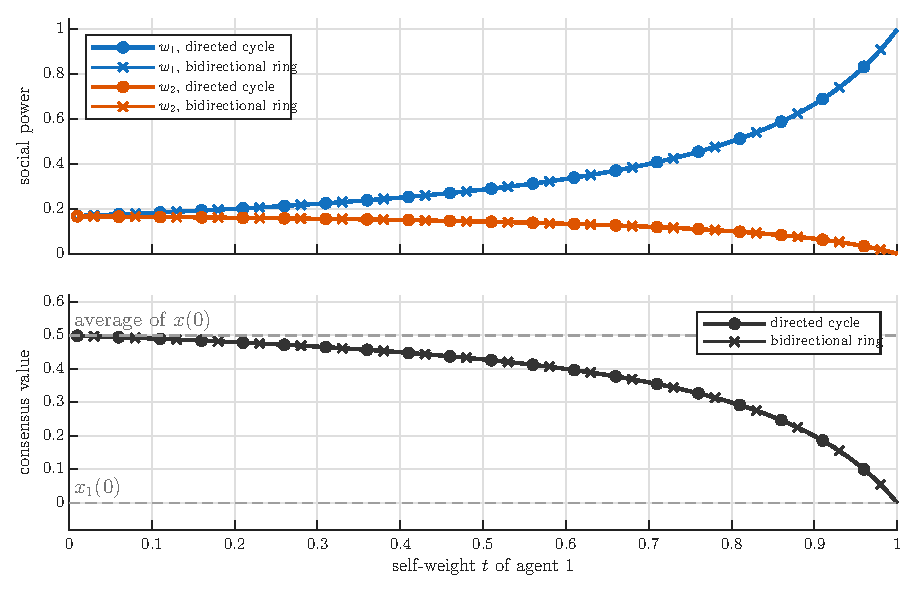
\includegraphics[width=0.94\textwidth]{figures/fdg_social_power.eps}
  \caption{Top: social power of agent~$1$ ($w_1$) and of agent~$2$ ($w_2$) as a
  function of the self-weight $t \in (0,1]$ of agent~$1$. Bottom: consensus value
  $w^\top x(0)$ for $x(0) = (0,\, 0.2,\, 0.4,\, 0.6,\, 0.8,\, 1)^\top$; the dashed
  lines mark the average of $x(0)$ and $x_1(0)$. Both panels are computed numerically
  in the directed cycle (dots) and in the bidirectional ring (crosses); the two networks
  give the same values.}
  \label{fig:fdg-power}
\end{figure}

\begin{remark}[More than one stubborn agent]
\label{rem:many-stubborn}
If two or more agents are stubborn, each of them is a sink of $C(G)$ made of a single,
aperiodic node. If every other agent is influenced, directly or through
intermediaries, by at least one stubborn agent, these are the only sinks, and by
Theorem~\ref{thm:disagreement} the group converges, but to a disagreement: every stubborn agent keeps its own initial opinion, and every other
agent converges to a convex combination of the opinions of the stubborn agents it is
influenced by (see also~\cite{proskurnikov2017tutorial}). Since there is no single
consensus value, the social power is no longer defined. This situation, in which
several agents are anchored to different fixed opinions, is the starting point of the
Friedkin--Johnsen model of Section~\ref{sec:fj}.
\end{remark}
